\makeatletter
\def\input@path{{../styles/}{../../styles/}{../../../styles/}{../}{../../}{../../../}}
\makeatother
\documentclass{ee122_notes}
% macros.tex - Course meta information
\renewcommand{\course}{EE 122} % with a space
\renewcommand{\coursetitle}{Introduction to Control Systems}
\renewcommand{\instructor}{Ayush Pandey}
\renewcommand{\student}{Name: }

\renewcommand{\semester}{Spring 2026}
\date{\semester} % this sets the LaTeX date field safely

% Problem set number
\renewcommand{\psetnum}{1}

% Release / due — use renewcommand because package provides empties
\renewcommand{\releasedate}{January 20, 2026}
\renewcommand{\duedate}{May 14, 2026}

% The following packages can be found on http:\\www.ctan.org
% \usepackage{graphics} % for pdf, bitmapped graphics files
%\usepackage{epsfig} % for postscript graphics files
%\usepackage{mathptmx} % assumes new font selection scheme installed
%\usepackage{times} % assumes new font selection scheme installed
\usepackage{amsmath} % assumes amsmath package installed
\usepackage{amssymb,mathtools}  % assumes amsmath package installed
\usepackage{xcolor}
\usepackage{pgfplots,subcaption}
\usepackage[hidelinks]{hyperref}
\usepackage{verbatim}
\usepackage{graphicx}
\usepackage{listings}
\usepackage{fancyhdr}
% \usepackage{geometry}
\usepackage{siunitx}
\usepackage[most]{tcolorbox}
\usepackage{enumitem}
\usepackage{environ}
\usepackage{pifont}
% -------- listings (Python) ----------
\lstdefinestyle{py}{
  language=Python,
  basicstyle=\ttfamily\small,
  keywordstyle=\color{blue!60!black}\bfseries,
  commentstyle=\color{green!40!black},
  stringstyle=\color{orange!60!black},
  showstringspaces=false,
  columns=fullflexible,
  frame=single,
  framerule=0.3pt,
  numbers=left,
  numberstyle=\tiny,
  xleftmargin=1em,
  tabsize=2,
  breaklines=true,
}

\usepackage[american]{circuitikz}
\usepackage{tikz}
\usetikzlibrary{arrows.meta,positioning,calc,angles,quotes}
\tikzset{
  >={Latex[length=2.2mm]},
  block/.style={draw, thick, rectangle, minimum height=10mm, minimum width=24mm, align=center},
  gain/.style={block, minimum width=14mm},
  sum/.style={draw, thick, circle, inner sep=0pt, minimum size=6mm},
  conn/.style={-Latex, thick},
}
\usepackage{caption}    
\usepackage{lscape}
\usepackage{soul}
\usepackage{physics}
\usepackage{hyperref}
\hypersetup{
    colorlinks=true,
    linkcolor=blue,
    filecolor=magenta,      
    urlcolor=blue,
    pdftitle={week1_notes},
    pdfpagemode=FullScreen,
}
%\usepackage{float} 

%\usepackage[demo]{graphicx}
\pgfplotsset{compat=1.18}
% \usepgfplotslibrary{fillbetween}

\newsavebox{\measurebox}

\let\proof\relax\let\endproof\relax


\def\abs#1{\left\lvert#1\right\rvert}
\let\proof\relax
\let\endproof\relax
\usepackage{amsthm}
\usepackage{accents}
\usepackage{relsize}
\newcommand{\ubar}[1]{\underaccent{\bar}{#1}}
\newtheorem{theorem}{Theorem}
\newtheorem{corollary}{Corollary}[theorem]
\newtheorem{lemma}{Lemma}
\newtheorem{proposition}{Proposition}
\newtheorem{statement}{Statement}

\theoremstyle{definition}
\newtheorem{definition}{Definition}
 
\theoremstyle{remark}
\newtheorem*{remark}{Remark}
\theoremstyle{remark}
\newtheorem*{claim}{Claim}
\setlength{\parindent}{0cm}
\newenvironment{nalign}{
    \begin{equation}
    \begin{aligned}
}{
    \end{aligned}
    \end{equation}
    \ignorespacesafterend
} 

\renewcommand{\releasedate}{January 28, 2026}
\begin{document}

\section*{EE 122/ME 141 Week 2, Lecture 2 (Spring 2026)}
\subsection*{Instructor: \instructor}
\subsection*{Date: \releasedate}
\section{Goals}
\begin{enumerate}
    \item Understand time-domain and frequency domain models of dynamical systems.
    \item Develop a state space representation from ordinary differential equations (ODEs), a time-domain model.
    \item Interpret properties of a system from its model with focus on second-order systems.
\end{enumerate}
\section{Recap: system models}
\begin{popquiz}
You see a mathematical model of a system as follows:
\[
\frac{dP}{dt} = kP\left(1-\frac{P}{L}\right)
\]
Select all options that are correct:
\begin{enumerate}
  \item This is a frequency-domain model computed using Fourier transforms.
  \item This is a transfer function in the Laplace domain.
  \item This is a time-domain model.
  \item The variable $P$ will change with time.
\end{enumerate}
\popqsplit

\textbf{Answer:} Options 3 and 4 are correct. This is a time-domain model (an ODE), and $P$ is explicitly a function of time $t$.
\end{popquiz}

\begin{popquiz}
Given a differential equation model of a system, $\frac{dy}{dt} + ky = -ut$, where $y$ is the output and $u$ is the input, which of the following is true?
\begin{enumerate}
  \item This is a time-domain model.
  \item The ODE is in frequency domain.
  \item The system is linear.
  \item The system is 1st-order.
  \item The system is 2nd-order.
\end{enumerate}
\popqsplit

\textbf{Answer:} Options 1, 3, and 4 are correct. This is a first-order time-domain ODE with linear dynamics.
\end{popquiz}

\begin{popquiz}
You have a model of a system as a transfer function:
\[
G(s) = \frac{5}{s(s+1)}
\]
Select all options that are true:
\begin{enumerate}
  \item The system model is in time-domain.
  \item The system model is in Laplace domain.
  \item The system is linear.
  \item The system is 2nd-order.
\end{enumerate}
\popqsplit
\textbf{Answer:} Options 2, 3, and 4 are correct. This is a Laplace domain transfer function, which represents a linear system. The denominator has degree 2, so the system is 2nd-order.
\end{popquiz}

\begin{popquiz}
True or False: A linear differential equation representation of a system can be transformed using Laplace transforms to get the system transfer function.
\popqsplit
\begin{enumerate}
  \item True
  \item False
\end{enumerate}

\textbf{Answer:} True. Taking the Laplace transform of a linear time-invariant differential equation (with zero initial conditions) yields the transfer function $G(s) = \frac{Y(s)}{U(s)}$, which relates the output to the input in the frequency domain.
\end{popquiz}

\section{Why Laplace transforms / transfer functions?}
After the previous lecture, did you wonder why we even introduce the Laplace transform and develop transfer functions? In this lecture, we will answer this question. Specifically, we will present two main reasons why we use Laplace domain models.
\section{Reason \#1: System response is easier to compute in Laplace domain} 
Consider a differential equation model of a second order system with input $u(t)$ and output $y(t)$:
\[
\frac{d^2 y}{dt^2} + 5 \frac{d y}{dt} + 6 y = u(t).
\]
You can think of the swing-down pendulum that you experimented with in the lab as an example of a real-world system that is modeled by a second-order ODE like this one. Now, let us assume that the input is a unit step: $u(t)=1$. The goal is:
% create blocked quote question:
\begin{quote}
\textbf{Question:} How do we compute the output $y(t)$ for $t>0$ given this input?
\end{quote}

\subsection{Approach 1: Solve the differential equation}
To solve the ODE directly (recall your linear algebra and differential equation class), we need to find the homogeneous solution (solution to the associated homogeneous equation) and a particular solution (any one solution that matches the forcing input). The total solution is the sum of these two components. Before we go any further, let us recall what these two components are and why we solve differential equations this way.

First, the differential equation is a linear equation, so the principle of superposition applies. This means that if $y_1(t)$ is a solution to the differential equation and $y_2(t)$ is another solution, then any linear combination of these two solutions is also a solution. So, to solve the differential equation given to us, we propose that we will break the solution down into two parts (to make the problem easier to solve): the equation with zero right-hand side, that is, with no input applied and the equation with the input applied. The first equation is called the homogeneous equation and its solution is called the homogeneous solution. Since no input is applied and we get a $y_h(t)$ that satisfies the homogeneous equation, we call this the \textbf{natural response} of the system. This is the way the system responds \emph{naturally} even when no input is applied and the system starts with some non-zero initial condition (similar to how you released the pendulum from a non-zero angle in the lab). Once you have the homogeneous solution, you can find a particular solution that matches the input applied. This is called the \textbf{forced response} of the system since it is driven by the input applied to the system. The total solution is the sum of these two components.

\subsection{The homogeneous solution}
To find the homogeneous solution, we set the right-hand side to zero:
\[
\frac{d^2 y_h}{dt^2} + 5 \frac{d y_h}{dt} + 6 y_h = 0.
\]
To solve this, we propose a solution of the form $y_h(t) = k e^{a t}$. We substitute this into the homogeneous equation, where each of the terms become:
\[
\frac{d^2 y_h}{dt^2} = k a^2 e^{a t}, \quad \frac{d y_h}{dt} = k a e^{a t}, \quad y_h = k e^{a t}.
\]
Substituting these into the homogeneous equation, we get:
\[
k a^2 e^{a t} + 5 k a e^{a t} + 6 k e^{a t} = 0.
\]
Factoring out $k e^{a t}$ (which is non-zero for all $t$), we get:
\[
k e^{a t} (a^2 + 5 a + 6) = 0.
\]
This implies that the term in parentheses must be zero:
\[
a^2 + 5 a + 6 = 0.
\]
To solve this quadratic equation, we can write it as \(a^2 + 2a + 3a + 6 = a (a + 2) + 3 (a + 2) = (a + 2)(a + 3) = 0\) and factor:
\[
a = -2, \quad a = -3.
\]
Thus, the homogeneous solution is:
\[
y_h(t) = k_1 e^{-2 t} + k_2 e^{-3 t},
\]
where $k_1$ and $k_2$ are constants determined by the initial conditions (we will do this later). We add the two exponential terms since the differential equation is linear and both terms are solutions to the homogeneous equation (you can try for yourself: substitute $e^{-2 t}$ into the homogeneous equation and verify that it satisfies the equation; do the same for $e^{-3 t}$).
\subsection{The particular solution}
To find the particular solution, we need to find a solution that matches the input applied. Since the input is a unit step, we can propose a constant solution for the particular solution: $y_p(t) = A$. Substituting this into the differential equation, we get:
\[
0 + 0 + 6 A = 1 \implies A = \frac{1}{6}.
\]
Thus, the particular solution is:
\[
y_p(t) = \frac{1}{6}.
\]
\subsection{The total solution}
The total solution is the sum of the homogeneous and particular solutions:
\[
y(t) = y_h(t) + y_p(t) = k_1 e^{-2 t} + k_2 e^{-3 t} + \frac{1}{6}.
\]
To find the constants $k_1$ and $k_2$, we need initial conditions. Let us assume that the system starts from rest, i.e., $y(0) = 0$ and $\frac{dy}{dt}(0) = 0$. Applying these initial conditions, we get:
\[
y(0) = k_1 + k_2 + \frac{1}{6} = 0 \implies k_1 + k_2 = -\frac{1}{6},
\]
and since the derivative is:
\[
\frac{dy}{dt} = -2 k_1 e^{-2 t} - 3 k_2 e^{-3 t},
\] 
we have:
\[
\frac{dy}{dt}(0) = -2 k_1 - 3 k_2 = 0 \implies 2 k_1 + 3 k_2 = 0.
\]
So, we have two equations with two unknowns:
\[
k_1 + k_2 = -\frac{1}{6}, \quad 2 k_1 + 3 k_2 = 0.
\]
Solving these equations, we find:
\[
k_1 = -\frac{1}{2}, \quad k_2 = \frac{1}{3}.
\]
So, we finally have the total solution:
\[
y(t) = -\frac{1}{2} e^{-2 t} + \frac{1}{3} e^{-3 t} + \frac{1}{6}.
\]

Now, let us try to solve the same equation by applying Laplace transform.
\subsection{Approach 2: Laplace transform}
Taking the Laplace transform of both sides of the differential equation (refer to the Laplace transform tables), we get:
\[
s^2 Y(s) - s y(0) - \frac{dy}{dt}(0) + 5 (s Y(s) - y(0)) + 6 Y(s) = U(s).
\]
Substituting the initial conditions $y(0) = 0$ and $\frac{dy}{dt}(0) = 0$, we get:
\[
(s^2 + 5 s + 6) Y(s) = U(s).
\]
For a unit step input, $U(s) = \frac{1}{s}$, so we have:
\[
Y(s) = \frac{1}{s (s^2 + 5 s + 6)}.
\]
To find $y(t)$, we need to take the inverse Laplace transform of $Y(s)$. We can use partial fraction decomposition to break down $Y(s)$:
\[
Y(s) = \frac{A}{s} + \frac{B}{s+2} + \frac{C}{s+3}.
\]
We can solve for $A$, $B$, and $C$ by multiplying both sides by the denominator and equating coefficients. We get 
\[
1 = A (s+2)(s+3) + B s (s+3) + C s (s+2).
\]
Setting $s=0$, we find $A = \frac{1}{6}$. Setting $s=-2$, we find $B = -\frac{1}{2}$. Setting $s=-3$, we find $C = \frac{1}{3}$. Thus, we have:
\[
Y(s) = \frac{1/6}{s} - \frac{1/2}{s+2} + \frac{1/3}{s+3}.
\]
Taking the inverse Laplace transform of each term (using Laplace transform tables), we get:
\[
y(t) = \frac{1}{6} - \frac{1}{2} e^{-2 t} + \frac{1}{3} e^{-3 t},
\]
which matches the solution we obtained by solving the differential equation directly. Mathematically, both approaches are equivalent. But once you know how to use Laplace transforms, you can see how Approach \#2 is much easier and straightforward -- we did not need to think about the homogeneous and particular solutions separately, and we did not need to worry about finding constants using initial conditions explicitly. The Laplace transform method handles all of that for us.

Here is a practice problem:
\begin{popquiz}
A second-order system has transfer function $G(s)=\frac{k}{s^2+2\zeta\omega_n s+\omega_n^2}$. Write an expression for $Y(s)$ for (i) an impulse input and (ii) a unit-step input.
\popqsplit
For an impulse, $U(s)=1$, so
\[
Y(s)=G(s)=\frac{k}{s^2+2\zeta\omega_n s+\omega_n^2}.
\]
For a unit step, $U(s)=1/s$, so
\[
Y(s)=\frac{k}{s\left(s^2+2\zeta\omega_n s+\omega_n^2\right)}.
\]
\end{popquiz}

\section{Reason \#2: Interpreting system properties}
By writing the transfer function, we get a quick peak into the characteristic system properties. So, for the transfer function we derived above, we have
\[
G(s) = \frac{1}{s^2 + 5 s + 6} = \frac{1}{(s+2)(s+3)}.
\]
Just by looking at the roots of the denominator, we can identify two important properties: (1) natural modes of the system occur at $s=-2$ and $s=-3$ because we can clearly see that the transfer function goes to infinity at these values of $s$ (these are special values, that, as we will learn later in the course, correspond to the system poles that describe the natural response of a system), and (2) since both roots have negative real parts, the system is stable (the natural response will decay to zero over time). You cannot see these properties as easily from the differential equation representation, especially when you have higher-order systems / complicated differential equations.

Let us analyze a physical system example next. 
\section{Example: A spring mass damper}
Second-order dynamics are everywhere: suspensions, doors, elevators, robots, and more. A spring mass damper system (see Figure~\ref{fig:spring_mass_damper}) is a classic model of a suspension system in a vehicle. Here, the output variable that you are interested in is the position of the vehicle and the input is the force applied by the road (and potential potholes) to the vehicle. Let us start by modeling the system from first-principles using Newton's laws of motion. 

\begin{figure}[h]
    \begin{center}
    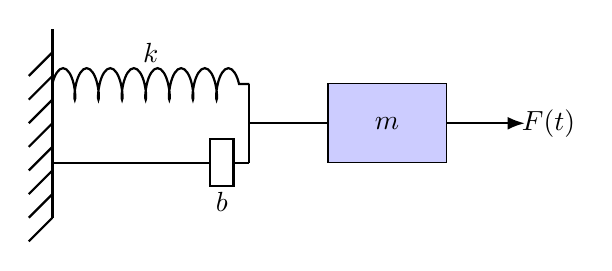
\begin{tikzpicture}
        % Draw the wall on the left
        \draw[thick] (0,0.3) -- (0,2.7);
        \draw[thick] (0,0.3) -- (-0.3,0);
        \draw[thick] (0,0.6) -- (-0.3,0.3);
        \draw[thick] (0,0.9) -- (-0.3,0.6);
        \draw[thick] (0,1.2) -- (-0.3,0.9);
        \draw[thick] (0,1.5) -- (-0.3,1.2);
        \draw[thick] (0,1.8) -- (-0.3,1.5);
        \draw[thick] (0,2.1) -- (-0.3,1.8);
        \draw[thick] (0,2.4) -- (-0.3,2.1);
        
        % Draw the spring (top)
        \draw[thick,decorate,decoration={coil,aspect=0.3,segment length=3mm,amplitude=2mm}] (0,2) -- (2.5,2);
        
        % Draw the damper (bottom) - piston symbol
        \draw[thick] (0,1) -- (2,1);
        \draw[thick] (2,0.7) rectangle (2.3,1.3);
        \draw[thick] (2.3,1) -- (2.5,1);
        
        % Connect spring and damper to mass
        \draw[thick] (2.5,2) -- (2.5,1.5);
        \draw[thick] (2.5,1) -- (2.5,1.5);
        \draw[thick] (2.5,1.5) -- (3.5,1.5);
        
        % Draw the mass
        \draw[fill=blue!20] (3.5,1) rectangle (5,2);
        \node at (4.25,1.5) {$m$};
        
        % Draw the external force arrow
        \draw[thick,->] (5,1.5) -- (6,1.5);
        \node at (6.3,1.5) {$F(t)$};
        
        % Add labels
        \node at (1.25,2.4) {$k$};
        \node at (2.15,0.5) {$b$};
        
    \end{tikzpicture}
    \caption{A spring-mass-damper system.}
    \label{fig:spring_mass_damper}
    \end{center}
\end{figure}

We can write the acceleration of the mass using Newton's second law ($F = ma$), with $p$ being the position of the mass:
\[
m \frac{d^2 p}{dt^2} = -k p - b \frac{d p}{dt} + F(t)
\]
where we have used the linear spring force $-k p$ and the damping force is dependent on the velocity $-b \frac{d p}{dt}$. Rearranging, we get:
\[
m \frac{d^2 p}{dt^2} + b \frac{d p}{dt} + k p = F(t).
\]
Taking the Laplace transform of both sides, we get:
\[
m s^2 P(s) + b s P(s) + k P(s) = F(s)
\]
which gives us the transfer function:
\[
G(s) = \frac{P(s)}{F(s)} = \frac{1}{m s^2 + b s + k} = \frac{\frac{1}{m}}{s^2 + \frac{b}{m} s + \frac{k}{m}}.
\]
We can rewrite this transfer function in the standard second-order form:
\[
G(s) = \frac{\omega_n^2}{s^2 + 2 \zeta \omega_n s + \omega_n^2},
\]
where
\[
\omega_n = \sqrt{\frac{k}{m}}, \quad \zeta = \frac{b}{2 m \omega_n} = \frac{b}{2 \sqrt{m k}}.
\]
Here, $\omega_n$ is called the \textbf{natural frequency} (units: rad/s) and $\zeta$ is called the \textbf{damping ratio} (dimensionless).
\textbf{Interpretation:} Two car suspensions can have the same damping ratio but different $\omega_n$. The one with larger $\omega_n$ responds faster and oscillates more rapidly. Damping describes how quickly oscillations die out. The dimensionless damping ratio $\zeta$ classifies the response:
\[
0<\zeta<1 \ \text{underdamped (oscillatory)}, \qquad
\zeta=1 \ \text{critically damped}, \qquad
\]
\[
\zeta>1 \ \text{overdamped (non-oscillatory)}.
\]

Here's how we use this in practice (an example): A door closer is designed to avoid oscillation. Its effective damping ratio is typically at or above $1$ so the door returns smoothly without bouncing!

\section{State-space representation}
We started with ODE representation of a system model --- a time-domain model. Then, we applied Laplace transform to get the transfer function representation --- a frequency-domain model. There is yet another way to represent dynamical systems: the state-space representation. This is also a time-domain model, but it is in a different form than the ODE representation. The state-space representation is suitable for describing complicated system dynamics in a manner that is easy to manipulate, while still being in the time-domain. Here, we write the dynamics using matrices and vectors. Let us write the spring mass damper dynamics in state-space form. 

What is a state that represents the spring mass damper system? The position $p(t)$ is one state. What else do we need to describe the system completely at any time $t$? We also need the velocity $\frac{d p}{dt}$, since the acceleration depends on both position and velocity. Thus, we define the state vector as:
\[
\mathbf{x}(t) = \begin{bmatrix} x_1(t) \\ x_2(t) \end{bmatrix} = \begin{bmatrix} p(t) \\ \frac{d p}{dt} \end{bmatrix}.
\]
The state-space representation consists of two equations: the state equation and the output equation. The state equation describes how the states evolve over time, and the output equation describes how the output is related to the states. For our spring mass damper system, we can re-write the ODE as:
\[
\ddot{p} = -\frac{k}{m} p - \frac{b}{m} \dot{p} + \frac{1}{m} F(t)
\]

So, we can write the state equations as:
\[
\frac{d}{dt} \begin{bmatrix} x_1(t) \\ x_2(t) \end{bmatrix} = \begin{bmatrix} \dot{x}_1(t) \\ \dot{x}_2(t) \end{bmatrix} = \begin{bmatrix} x_2(t) \\ -\frac{k}{m} x_1(t) - \frac{b}{m} x_2(t) + \frac{1}{m} F(t) \end{bmatrix}.
\]
We can express this in matrix form as:
\[
\frac{d \mathbf{x}(t)}{dt} = \begin{bmatrix} 0 & 1 \\ -\frac{k}{m} & -\frac{b}{m} \end{bmatrix} \mathbf{x}(t) + \begin{bmatrix} 0 \\ \frac{1}{m} \end{bmatrix} F(t).
\]
The output equation relates the output (position $p(t)$) to the states:
\[
y(t) = \begin{bmatrix} 1 & 0 \end{bmatrix} \mathbf{x}(t).
\]

Thus, the state-space representation of the spring mass damper system is:
\[ \dot{x} = Ax + Bu \quad y = Cx + Du \]
where
\[
A = \begin{bmatrix} 0 & 1 \\ -\frac{k}{m} & -\frac{b}{m} \end{bmatrix}, \quad B = \begin{bmatrix} 0 \\ \frac{1}{m} \end{bmatrix}, \quad C = \begin{bmatrix} 1 & 0 \end{bmatrix}, \quad D = 0.
\]
We will explore state-space representation in more detail in future lectures. Here's a food for thought until then: the eigenvalues of the state matrix $A$ are the same as the poles of the transfer function $G(s)$!

\end{document}